\documentclass[12pt,a4paper]{scrartcl}\usepackage[]{graphicx}\usepackage[]{color}
% maxwidth is the original width if it is less than linewidth
% otherwise use linewidth (to make sure the graphics do not exceed the margin)
\makeatletter
\def\maxwidth{ %
  \ifdim\Gin@nat@width>\linewidth
    \linewidth
  \else
    \Gin@nat@width
  \fi
}
\makeatother

\definecolor{fgcolor}{rgb}{0.345, 0.345, 0.345}
\newcommand{\hlnum}[1]{\textcolor[rgb]{0.686,0.059,0.569}{#1}}%
\newcommand{\hlstr}[1]{\textcolor[rgb]{0.192,0.494,0.8}{#1}}%
\newcommand{\hlcom}[1]{\textcolor[rgb]{0.678,0.584,0.686}{\textit{#1}}}%
\newcommand{\hlopt}[1]{\textcolor[rgb]{0,0,0}{#1}}%
\newcommand{\hlstd}[1]{\textcolor[rgb]{0.345,0.345,0.345}{#1}}%
\newcommand{\hlkwa}[1]{\textcolor[rgb]{0.161,0.373,0.58}{\textbf{#1}}}%
\newcommand{\hlkwb}[1]{\textcolor[rgb]{0.69,0.353,0.396}{#1}}%
\newcommand{\hlkwc}[1]{\textcolor[rgb]{0.333,0.667,0.333}{#1}}%
\newcommand{\hlkwd}[1]{\textcolor[rgb]{0.737,0.353,0.396}{\textbf{#1}}}%
\let\hlipl\hlkwb

\usepackage{framed}
\makeatletter
\newenvironment{kframe}{%
 \def\at@end@of@kframe{}%
 \ifinner\ifhmode%
  \def\at@end@of@kframe{\end{minipage}}%
  \begin{minipage}{\columnwidth}%
 \fi\fi%
 \def\FrameCommand##1{\hskip\@totalleftmargin \hskip-\fboxsep
 \colorbox{shadecolor}{##1}\hskip-\fboxsep
     % There is no \\@totalrightmargin, so:
     \hskip-\linewidth \hskip-\@totalleftmargin \hskip\columnwidth}%
 \MakeFramed {\advance\hsize-\width
   \@totalleftmargin\z@ \linewidth\hsize
   \@setminipage}}%
 {\par\unskip\endMakeFramed%
 \at@end@of@kframe}
\makeatother

\definecolor{shadecolor}{rgb}{.97, .97, .97}
\definecolor{messagecolor}{rgb}{0, 0, 0}
\definecolor{warningcolor}{rgb}{1, 0, 1}
\definecolor{errorcolor}{rgb}{1, 0, 0}
\newenvironment{knitrout}{}{} % an empty environment to be redefined in TeX

\usepackage{alltt}
\usepackage[utf8]{inputenc}
\usepackage{amsmath}
\usepackage{graphicx}
\usepackage{tikz}
%\usepackage{silence}
\usepackage{mdframed}
%\WarningFilter{mdframed}{You got a bad break}
\usepackage[colorinlistoftodos]{todonotes}
\usepackage{listings}
\usepackage{color}
\colorlet{exampcol}{blue!10}
\usepackage{multicol}
\usepackage{booktabs}


\usepackage{setspace}
%\doublespacing

\usepackage[noanswer]{exercise}%[noanswer]
\renewcommand{\ExerciseHeaderTitle}{\quad---\quad \color{orange!70!black}\ExerciseTitle}


\usepackage[autostyle, english = american]{csquotes}
\MakeOuterQuote{"}

\usepackage{hyperref}
\hypersetup{
    colorlinks,
    citecolor=black,
    filecolor=black,
    linkcolor=blue,
    urlcolor=blue
}

\title{R-StatProgamming with functions in R}
\date{\today}
\author{Timoth\'ee Bonnet, BDSI}
\IfFileExists{upquote.sty}{\usepackage{upquote}}{}
\begin{document}



\maketitle

On Friday 20/03/2020 I will be presenting this tutorial live on Zoom. (ask by email/Slack if you do not know how to use Zoom.)

If you have any trouble going through this tutorial then or at a different time you can chat about it on Slack ( rsb-r-stats-biology.slack.com , if you are not a member but would like to be, drop me an email) or email me at \href{mailto:timotheebonnetc@gmail.com}{timotheebonnetc@gmail.com}.

If you do not attend the Zoom meeting but would like to receive credit through the \href{https://wattlecourses.anu.edu.au/enrol/index.php?id=23938}{COS Career Development Framework} program I need you to complete three exercises of your choice. Send me your answers via Slack or email. It does not have to be correct on the first try and you are welcome to get in touch if you are completely stuck. I will provide feedback to help you complete exercises you want to do.

In this tutorial you will learn:

\begin{itemize}
    \item What is a function in R.
    \item Why it is useful to make your own functions.
    \item How to make a function.
\end{itemize}

\tableofcontents
\ListOfExerciseInToc
\ExerciseLevelInToc{subsubsection}

\clearpage



\section{What is a function?}

A function is a piece of code, possibly long and complex, that is saved as an object in R, so that you can access this code using a single word.

You can see the code invoked by a function by running the function name without parentheses. For instance try to run:
\begin{knitrout}
\definecolor{shadecolor}{rgb}{0.969, 0.969, 0.969}\color{fgcolor}\begin{kframe}
\begin{alltt}
\hlstd{tapply}
\end{alltt}
\end{kframe}
\end{knitrout}
So, over 30 lines of complex code are run when you call this function.

In R, most \textbf{functions take some arguments (=input objects) and return one output}.
For instance, the function \texttt{mean()} takes a numeric vector as arguments and return a number as output:
\begin{knitrout}
\definecolor{shadecolor}{rgb}{0.969, 0.969, 0.969}\color{fgcolor}\begin{kframe}
\begin{alltt}
\hlstd{input} \hlkwb{<-} \hlkwd{c}\hlstd{(}\hlnum{1}\hlstd{,}\hlnum{3}\hlstd{,}\hlnum{5}\hlstd{,}\hlnum{10}\hlstd{)} \hlcom{# create a vector of numbers}
\hlkwd{mean}\hlstd{(input)} \hlcom{# output the mean of that vector}
\end{alltt}
\begin{verbatim}
## [1] 4.75
\end{verbatim}
\end{kframe}
\end{knitrout}
It is much more efficient to call the function mean than to write a piece of code calculating the mean of that vector using addition and division.

If you want to know what a function does and what type of input it requires look at its help page (every function coming from R-base or CRAN packages should have a help page). You can look for this page on a web browser (for instance type \texttt{mean() R}), search the function name in the \texttt{Help} tab of R-Studio, type \texttt{?mean}, or start press \texttt{tab} when your cursor is between the parentheses of \texttt{mean()}.

Many functions can take more than one arguments. How does the function what is what? There are two complementary ways:
\begin{enumerate}
\item By order: the help page of each function shows you in which order arguments are expected. For instance \texttt{mean(1:4, 0, FALSE)}.
\item By name: direct a value to a specific argument using \texttt{name = value}. When you call some arguments by name, the order in which they appear within the function call does not matter. For instance \texttt{mean(trim=0, x=1:4, na.rm=FALSE)}
\end{enumerate}
You can mix the two, for instance: \texttt{mean(1:4, na.rm=FALSE, trim=0)}.
It is safer to use argument names and I recommend you use this approach unless you are just writing quick code that you will not reuse or you know the functions you are using very well.

One last thing: functions can have default values for their arguments; that is, values that will be use if you do not provide a value for that argument. For instance \texttt{mean()} has a default value for the arguments \texttt{trim} and \texttt{na.rm} but not for \texttt{x}. You absolutely need to provide a value for \texttt{x} or the function will return an error message. You can find which arguments have default values on the function help page, in the section Usage: arguments with default values are followed by \texttt{=} and the default value in the function call, for instance \texttt{mean(x, trim = 0, na.rm = FALSE, ...)}.



If you are curious, there is a more advanced description of what functions really are in R at \url{https://adv-r.hadley.nz/functions.html} (you probably do not need this information, unless you want to become an R wizard.).

\section{Why and how make your own functions?}

There are lots of functions available in R-base and R-packages, so why bother? If you think you are going a piece of code only once and no one else will ever use your code, then don't bother. But if there is a chance you need to run the same series of commands multiple times, it very quickly becomes faster, cleaner and safer to turn your code into a function. 

For instance, imagine you have 20 data sets on which you want to apply some data transformation, run some statistical tests, plot model predictions and write that plot to a .png file to use in a report. That series of operations may be 15 lines long. If you copy paste the code for each data set you will need 300 lines of code and are likely to make typos that may be difficult to find. If you write your code as a function, you may need 20 lines of code (in general it will), but then you can analyse each data set in 1 line. In total you will need 40 lines instead of 300. 
Further, if you decide to change the statistical model later on, you need to modify your code in only one spot, inside the function. You probably will not need to edit the 20 function calls for each data set.
Finally, writing functions will force you to make your code more robust (because it must work with slightly different input) which makes it less error prone and more easy to re-use and share with others. 

To keep your scripts clean, you can save all the functions you create for a given project into a single .R file, separate from your script doing your actual analyses. At the start of your analysis script you can source the function script in a way similar to loading packages using library.
For instance, if you save all your functions for a given project in the file MyFunctions.R, start the script where you will do your analyses by \texttt{source(MyFunctions.R)}.


NB: Building your own functions and sourcing them is similar to building your own package. In fact, once you have functions in a file it is quite simple to create an R-package (but we will see that another time).

\subsection{How to define a function}
To create a function, you need to assign the output of the function \texttt{function()} to an object\dots yes that is confusing, so here is an example.
Let’s start by defining a function fahrenheit\_to\_celsius that converts temperatures from Fahrenheit to Celsius:

\begin{knitrout}
\definecolor{shadecolor}{rgb}{0.969, 0.969, 0.969}\color{fgcolor}\begin{kframe}
\begin{alltt}
\hlstd{fahrenheit_to_celsius} \hlkwb{<-} \hlkwa{function}\hlstd{(}\hlkwc{temp_F}\hlstd{) \{}
  \hlstd{temp_C} \hlkwb{<-} \hlstd{(temp_F} \hlopt{-} \hlnum{32}\hlstd{)} \hlopt{*} \hlnum{5} \hlopt{/} \hlnum{9}
  \hlkwd{return}\hlstd{(temp_C)}
\hlstd{\}}
\end{alltt}
\end{kframe}
\end{knitrout}

After running this code, the function fahrenheit\_to\_celsius exists in your environment and you can use it:
\begin{knitrout}
\definecolor{shadecolor}{rgb}{0.969, 0.969, 0.969}\color{fgcolor}\begin{kframe}
\begin{alltt}
\hlkwd{fahrenheit_to_celsius}\hlstd{(}\hlnum{99}\hlstd{)}
\end{alltt}
\begin{verbatim}
## [1] 37.22
\end{verbatim}
\begin{alltt}
\hlkwd{fahrenheit_to_celsius}\hlstd{(}\hlnum{451}\hlstd{)}
\end{alltt}
\begin{verbatim}
## [1] 232.8
\end{verbatim}
\end{kframe}
\end{knitrout}


Look again at the code defining the function. Everything within \texttt{\{\}} is the code you run. Notice how the name of the argument (\texttt{temp\_F}) is used for a variable inside the function. Arguments are assigned to variables and that is how the code inside the function returns different values when you use different argument values.
What is inside \texttt{return()} is your function output. In R, if you do not write a \texttt{return()} in your function, the last command within your function will be returned as the output. I recommend you always use \texttt{return()} to be sure you know what your function outputs. 

\begin{Exercise}[difficulty=1, title={Build a first function}]
Write a function that return the product of three arbitrary numbers together (x*y*z) provided by the user.
\end{Exercise}
\begin{Answer}
\begin{knitrout}
\definecolor{shadecolor}{rgb}{0.969, 0.969, 0.969}\color{fgcolor}\begin{kframe}
\begin{alltt}
\hlstd{myfunction} \hlkwb{<-} \hlkwa{function}\hlstd{(}\hlkwc{x}\hlstd{,}\hlkwc{y}\hlstd{,}\hlkwc{z}\hlstd{)\{}
  \hlkwd{return}\hlstd{(x}\hlopt{*}\hlstd{y}\hlopt{*}\hlstd{z)}
\hlstd{\}}
\hlkwd{myfunction}\hlstd{(}\hlnum{100}\hlstd{,}\hlnum{2}\hlstd{,} \hlopt{-}\hlnum{0.005}\hlstd{)}
\end{alltt}
\begin{verbatim}
## [1] -1
\end{verbatim}
\end{kframe}
\end{knitrout}
\end{Answer}

The \texttt{return()} function (yes, it is a function itself!) can output a single object, but often we want to calculate many things at once, not just a single number! So how do you do if you want two or more values out of your function? 
Remember that in R, objects can be vectors, matrices, lists, data-frames\dots all of which can contain many values, possibly of different types. So you could very well write on object containing several values within your function and include that object within \texttt{return()}.


\begin{Exercise}[difficulty=2, title={Multiple values in output}]
Write a function that return the product of three arbitrary numbers together (x*y*z) as well as their sum (x+y+z). Remeber you can create vectors of several values using the function \texttt{c(x,y)}.
\end{Exercise}
\begin{Answer}
\begin{knitrout}
\definecolor{shadecolor}{rgb}{0.969, 0.969, 0.969}\color{fgcolor}\begin{kframe}
\begin{alltt}
\hlstd{myfunction} \hlkwb{<-} \hlkwa{function}\hlstd{(}\hlkwc{x}\hlstd{,}\hlkwc{y}\hlstd{,}\hlkwc{z}\hlstd{)\{}
  \hlkwd{return}\hlstd{(}\hlkwd{c}\hlstd{(x}\hlopt{*}\hlstd{y}\hlopt{*}\hlstd{z, x}\hlopt{+}\hlstd{y}\hlopt{+}\hlstd{z))}
\hlstd{\}}
\hlkwd{myfunction}\hlstd{(}\hlnum{100}\hlstd{,}\hlnum{2}\hlstd{,} \hlopt{-}\hlnum{0.005}\hlstd{)}
\end{alltt}
\begin{verbatim}
## [1]  -1 102
\end{verbatim}
\end{kframe}
\end{knitrout}
\end{Answer}


\begin{Exercise}[difficulty=2, title={Write a data-frame of random values in output}]
Write a function that return a data-frame containing 3 columns of randomly generated normal numbers (use the function \texttt{rnorm}). Your function should have an argument to control how many rows the data-frames has. As a bonus, create arguments to control the mean and standard deviation of each column.
\end{Exercise}
\begin{Answer}
\begin{knitrout}
\definecolor{shadecolor}{rgb}{0.969, 0.969, 0.969}\color{fgcolor}\begin{kframe}
\begin{alltt}
\hlstd{randomdf} \hlkwb{<-} \hlkwa{function}\hlstd{(}\hlkwc{rows}\hlstd{=}\hlnum{10}\hlstd{)\{}
  \hlstd{out} \hlkwb{<-} \hlkwd{data.frame}\hlstd{(}\hlkwc{x} \hlstd{=} \hlkwd{rnorm}\hlstd{(}\hlkwc{n}\hlstd{=rows),} \hlkwc{y}\hlstd{=} \hlkwd{rnorm}\hlstd{(}\hlkwc{n}\hlstd{=rows),} \hlkwc{z} \hlstd{=} \hlkwd{rnorm}\hlstd{(}\hlkwc{n}\hlstd{=rows))}
  \hlkwd{return}\hlstd{(out)}
\hlstd{\}}
\hlkwd{randomdf}\hlstd{(}\hlnum{100}\hlstd{)}
\end{alltt}
\begin{verbatim}
##            x         y        z
## 1   -1.73256 -0.381416  0.26776
## 2   -1.20891 -1.161080  0.94842
## 3   -0.29290  0.951413  0.21647
## 4    0.58344 -0.094548 -0.07972
## 5   -2.29534 -1.996447  0.19917
## 6   -1.64433  1.777070 -0.26480
## 7    0.55514  1.261519  0.27226
## 8    0.12480  1.051468 -1.22299
## 9    0.04621 -0.678801 -1.71999
## 10  -0.96199  0.280294  0.78574
## 11   2.78498  1.161394  0.39690
## 12  -1.31320 -0.094711 -0.44507
## 13   1.26908 -0.965803  0.98701
## 14  -0.59846 -1.178821 -0.88761
## 15   0.66865 -0.028865 -0.61844
## 16  -1.70428 -1.362641  2.03737
## 17   0.05416  0.731330  1.16949
## 18   0.13773 -1.496568 -0.35807
## 19   0.05730 -0.590597  0.90811
## 20  -0.59035 -1.743236  0.31156
## 21  -0.44490 -0.587844 -0.89732
## 22   1.36260 -0.014635 -0.50156
## 23  -1.74891  1.699269 -0.31322
## 24  -1.15198 -0.139901  0.73111
## 25   0.85298  2.161575 -0.14472
## 26  -1.00667  0.718445 -0.70608
## 27  -0.86490  1.164221  0.73248
## 28   1.79558  0.916162 -0.41942
## 29   0.33688  1.016571  0.52869
## 30  -0.40738 -0.691105 -2.04670
## 31   0.10463  0.129882 -1.85023
## 32  -0.75001 -1.437764  0.10999
## 33  -0.32791 -0.804544  0.82421
## 34  -0.23941  0.590249 -1.39228
## 35  -1.80582  0.583481  0.81046
## 36  -0.65201  0.318917  0.58190
## 37  -1.48327 -0.319986  0.34981
## 38   0.20400 -2.029747  0.87079
## 39  -0.12276  0.062123  1.18532
## 40  -2.08195 -0.444032 -0.31773
## 41  -0.47576  0.929292  1.29858
## 42   0.50781  0.069547  1.52422
## 43   0.69910 -1.061178 -0.64453
## 44  -1.29391  0.750027 -0.36947
## 45  -0.99683 -1.066229  1.40490
## 46  -0.31837  0.351576  0.68160
## 47   0.98017 -1.122722 -0.11650
## 48  -0.61037  0.033030 -0.87571
## 49   1.45158 -0.038225 -2.17670
## 50   0.23826  1.083685  0.19010
## 51  -0.59826 -1.326508  1.02648
## 52   0.21852 -0.418499 -0.18996
## 53   0.88362  1.041678 -0.26563
## 54  -1.10746  0.711368  0.72211
## 55  -0.13422  0.704568 -1.43978
## 56   1.47479  0.413209  2.22843
## 57  -1.10909 -1.659692  0.35054
## 58   0.20781 -0.557447  1.82341
## 59  -0.81788  0.532446 -0.50849
## 60  -0.97659  1.426673  0.90478
## 61   0.36598 -0.530964  0.98344
## 62   0.53876 -0.098635  0.39511
## 63  -0.92742  1.126397 -1.75467
## 64  -0.88465  1.062611 -0.90060
## 65  -0.12217 -0.871451 -1.66604
## 66   0.64997 -1.841077 -1.05001
## 67   0.58080  0.627677 -0.14367
## 68  -1.34080  1.185583 -0.51399
## 69   1.24875 -1.828849  0.01843
## 70   0.59931  0.622156  0.68648
## 71   0.69245  0.367755  0.12464
## 72   2.78454 -1.546402  0.74753
## 73  -0.11420 -0.287266 -0.93767
## 74  -2.19212 -1.342376  0.07403
## 75   0.94639  0.916187 -0.61794
## 76   0.23624 -0.189309 -0.34005
## 77  -0.85738  0.667433  0.81641
## 78   0.62266 -0.783324 -0.46101
## 79   1.07080 -0.830173  1.21634
## 80  -0.10068  1.785633  0.35748
## 81  -0.14877 -0.534302 -0.12105
## 82  -1.76240 -2.243027  0.23274
## 83   0.45244 -1.002291 -0.14599
## 84   0.41811 -0.196153  1.61870
## 85  -0.31058 -1.183375  1.40308
## 86   0.39515 -0.481543 -0.60494
## 87   0.07158 -1.011408  0.16995
## 88  -1.96808 -0.004938  0.39066
## 89  -0.67668  0.539405  1.02884
## 90  -0.23388 -1.197442  0.07878
## 91  -0.87688  1.246191  0.88945
## 92   0.40489 -1.698260  0.53993
## 93  -0.29365  0.024090 -1.16138
## 94  -0.25006 -0.041758 -1.44752
## 95  -0.75866 -0.443960  0.71189
## 96  -0.34393 -1.242983  1.20677
## 97  -1.19251 -1.111189  0.05432
## 98  -0.09405  1.236225 -0.98071
## 99  -1.18308  0.074687 -2.30874
## 100  0.52628 -0.539940 -0.26508
\end{verbatim}
\end{kframe}
\end{knitrout}
\end{Answer}
\clearpage

\subsection{Combining functions}

The real power of functions comes from mixing, matching and combining them into ever-larger chunks to get the effect we want.

Let’s define two functions that will convert temperature from Fahrenheit to Kelvin, and Kelvin to Celsius:

\begin{knitrout}
\definecolor{shadecolor}{rgb}{0.969, 0.969, 0.969}\color{fgcolor}\begin{kframe}
\begin{alltt}
\hlstd{fahr_to_kelvin} \hlkwb{<-} \hlkwa{function}\hlstd{(}\hlkwc{temp}\hlstd{) \{}
  \hlstd{kelvin} \hlkwb{<-} \hlstd{((temp} \hlopt{-} \hlnum{32}\hlstd{)} \hlopt{*} \hlstd{(}\hlnum{5} \hlopt{/} \hlnum{9}\hlstd{))} \hlopt{+} \hlnum{273.15}
  \hlkwd{return}\hlstd{(kelvin)}
\hlstd{\}}

\hlstd{kelvin_to_celsius} \hlkwb{<-} \hlkwa{function}\hlstd{(}\hlkwc{temp}\hlstd{) \{}
  \hlstd{celsius} \hlkwb{<-} \hlstd{temp} \hlopt{-} \hlnum{273.15}
  \hlkwd{return}\hlstd{(celsius)}
\hlstd{\}}
\end{alltt}
\end{kframe}
\end{knitrout}

We can define a function to convert directly from Fahrenheit to Celsius, by reusing these two functions above:

\begin{knitrout}
\definecolor{shadecolor}{rgb}{0.969, 0.969, 0.969}\color{fgcolor}\begin{kframe}
\begin{alltt}
\hlstd{fahr_to_celsius} \hlkwb{<-} \hlkwa{function}\hlstd{(}\hlkwc{temp}\hlstd{) \{}
  \hlstd{temp_k} \hlkwb{<-} \hlkwd{fahr_to_kelvin}\hlstd{(temp)}
  \hlstd{result} \hlkwb{<-} \hlkwd{kelvin_to_celsius}\hlstd{(temp_k)}
  \hlkwd{return}\hlstd{(result)}
\hlstd{\}}
\end{alltt}
\end{kframe}
\end{knitrout}

\begin{Exercise}[difficulty=2, title={Combine several functions together}]

Let's say you want to better understand the statistical properties of models you are using on real data. You would like to simulate data of known properties, fit models on these simulated data and visualize if you recover the truth in your data (match between expected and estimated values). That is all a bit complicated so you split the process in several functions. 
Below I give you working functions for each sub-task. Reuse these functions to create a short function running the whole process at once. Then play with parameter values (beta1 and beta2) and see what happens.

First you simulate data:
\begin{knitrout}
\definecolor{shadecolor}{rgb}{0.969, 0.969, 0.969}\color{fgcolor}\begin{kframe}
\begin{alltt}
\hlstd{simul_function} \hlkwb{<-} \hlkwa{function}\hlstd{(}\hlkwc{nbdatasets} \hlstd{=} \hlnum{10}\hlstd{,} \hlkwc{nbsamples}\hlstd{=} \hlnum{500}\hlstd{,} \hlkwc{alpha}\hlstd{=}\hlnum{1}\hlstd{,}
                           \hlkwc{beta1}\hlstd{=}\hlnum{0.5}\hlstd{,} \hlkwc{beta2}\hlstd{=}\hlopt{-}\hlnum{0.5}\hlstd{)}
\hlstd{\{}
  \hlstd{alldat} \hlkwb{<-} \hlkwd{list}\hlstd{()}
  \hlkwa{for} \hlstd{(i} \hlkwa{in} \hlnum{1}\hlopt{:}\hlstd{nbdatasets)}
  \hlstd{\{}
    \hlstd{x1} \hlkwb{<-} \hlkwd{rnorm}\hlstd{(}\hlkwc{n} \hlstd{= nbsamples)}
    \hlstd{x2} \hlkwb{<-} \hlstd{x1} \hlopt{+} \hlkwd{rnorm}\hlstd{(}\hlkwc{n} \hlstd{= nbsamples)}
    \hlstd{y} \hlkwb{<-} \hlstd{alpha} \hlopt{+} \hlstd{beta1}\hlopt{*}\hlstd{x1} \hlopt{+} \hlstd{beta2}\hlopt{*}\hlstd{x2} \hlopt{+} \hlkwd{rnorm}\hlstd{(}\hlkwc{n} \hlstd{= nbsamples)}
    \hlstd{alldat[[i]]} \hlkwb{<-} \hlkwd{data.frame}\hlstd{(}\hlkwc{x1}\hlstd{=x1,} \hlkwc{x2}\hlstd{=x2,} \hlkwc{y}\hlstd{=y)}
  \hlstd{\}}
  \hlkwd{return}\hlstd{(alldat)}
\hlstd{\}}\hlcom{#end simul_function()}

\hlstd{datexmple} \hlkwb{<-} \hlkwd{simul_function}\hlstd{()}
\end{alltt}
\end{kframe}
\end{knitrout}

Then you fit different models and extract parameter estimates.
\begin{knitrout}
\definecolor{shadecolor}{rgb}{0.969, 0.969, 0.969}\color{fgcolor}\begin{kframe}
\begin{alltt}
\hlstd{models_function} \hlkwb{<-} \hlkwa{function}\hlstd{(}\hlkwc{dat}\hlstd{)}
\hlstd{\{}
  \hlstd{res} \hlkwb{<-} \hlkwd{data.frame}\hlstd{(}\hlkwc{model1_alpha}\hlstd{=}\hlkwd{rep}\hlstd{(}\hlnum{NA}\hlstd{,}\hlkwc{times}\hlstd{=}\hlkwd{length}\hlstd{(dat)),}
                          \hlkwc{model1_beta1}\hlstd{=}\hlnum{NA}\hlstd{,} \hlkwc{model1_beta2}\hlstd{=}\hlnum{NA}\hlstd{,}
                          \hlkwc{model2_alpha}\hlstd{=}\hlkwd{rep}\hlstd{(}\hlnum{NA}\hlstd{,}\hlkwc{times}\hlstd{=}\hlkwd{length}\hlstd{(dat)),}
                          \hlkwc{model2_beta1}\hlstd{=}\hlnum{NA}\hlstd{,} \hlkwc{model2_beta2}\hlstd{=}\hlnum{NA}\hlstd{)}
  \hlkwa{for}\hlstd{(i} \hlkwa{in} \hlnum{1}\hlopt{:}\hlkwd{length}\hlstd{(dat))}
  \hlstd{\{}
    \hlstd{model1} \hlkwb{<-} \hlkwd{lm}\hlstd{(y} \hlopt{~} \hlstd{x1} \hlopt{+} \hlstd{x2,} \hlkwc{data} \hlstd{= dat[[i]])}

    \hlstd{model2} \hlkwb{<-} \hlkwd{lm}\hlstd{(y} \hlopt{~} \hlstd{x1,} \hlkwc{data} \hlstd{= dat[[i]])}

    \hlstd{model2bis} \hlkwb{<-} \hlkwd{lm}\hlstd{(}\hlkwd{residuals}\hlstd{(model2)} \hlopt{~} \hlstd{dat[[i]]}\hlopt{$}\hlstd{x2)}

    \hlstd{res[i,]} \hlkwb{<-} \hlkwd{c}\hlstd{(}\hlkwd{coef}\hlstd{(model1),} \hlkwd{coef}\hlstd{(model2),} \hlkwd{coef}\hlstd{(model2bis)[}\hlnum{2}\hlstd{])}
  \hlstd{\}}
  \hlkwd{return}\hlstd{(res)}
\hlstd{\}}\hlcom{#end models_function()}

\hlstd{modelresults} \hlkwb{<-} \hlkwd{models_function}\hlstd{(datexmple)}
\end{alltt}
\end{kframe}
\end{knitrout}

Finally you make boxplots out of pairs of parameter estimates and draw a red line showing the true value used during the simulation.
\begin{knitrout}
\definecolor{shadecolor}{rgb}{0.969, 0.969, 0.969}\color{fgcolor}\begin{kframe}
\begin{alltt}
\hlstd{visu_function} \hlkwb{<-} \hlkwa{function}\hlstd{(}\hlkwc{modelsoutput}\hlstd{,} \hlkwc{truevalues} \hlstd{=} \hlkwd{c}\hlstd{(}\hlnum{1}\hlstd{,} \hlnum{0.5}\hlstd{,} \hlopt{-}\hlnum{0.5}\hlstd{))}
\hlstd{\{}
  \hlkwd{par}\hlstd{(}\hlkwc{mfrow}\hlstd{=}\hlkwd{c}\hlstd{(}\hlnum{1}\hlstd{,}\hlnum{3}\hlstd{))}
  \hlkwd{boxplot}\hlstd{(modelsoutput[,}\hlkwd{c}\hlstd{(}\hlnum{1}\hlstd{,}\hlnum{4}\hlstd{)],} \hlkwc{main}\hlstd{=} \hlstr{"Alpha"}\hlstd{,}
          \hlkwc{names} \hlstd{=} \hlkwd{c}\hlstd{(}\hlstr{"model1"}\hlstd{,} \hlstr{"model2"}\hlstd{))}
  \hlkwd{abline}\hlstd{(}\hlkwc{h}\hlstd{=truevalues[}\hlnum{1}\hlstd{],} \hlkwc{col}\hlstd{=}\hlstr{"red"}\hlstd{)}

  \hlkwd{boxplot}\hlstd{(modelsoutput[,}\hlkwd{c}\hlstd{(}\hlnum{2}\hlstd{,}\hlnum{5}\hlstd{)],} \hlkwc{main}\hlstd{=} \hlstr{"Beta1"}\hlstd{,}
          \hlkwc{names} \hlstd{=} \hlkwd{c}\hlstd{(}\hlstr{"model1"}\hlstd{,} \hlstr{"model2"}\hlstd{))}
  \hlkwd{abline}\hlstd{(}\hlkwc{h}\hlstd{=truevalues[}\hlnum{2}\hlstd{],} \hlkwc{col}\hlstd{=}\hlstr{"red"}\hlstd{)}

  \hlkwd{boxplot}\hlstd{(modelsoutput[,}\hlkwd{c}\hlstd{(}\hlnum{3}\hlstd{,}\hlnum{6}\hlstd{)],} \hlkwc{main}\hlstd{=} \hlstr{"Beta2"}\hlstd{,}
          \hlkwc{names} \hlstd{=} \hlkwd{c}\hlstd{(}\hlstr{"model1"}\hlstd{,} \hlstr{"model2"}\hlstd{))}
  \hlkwd{abline}\hlstd{(}\hlkwc{h}\hlstd{=truevalues[}\hlnum{3}\hlstd{],} \hlkwc{col}\hlstd{=}\hlstr{"red"}\hlstd{)}
\hlstd{\}}\hlcom{#end visu_function}

\hlkwd{visu_function}\hlstd{(modelresults)}
\end{alltt}
\end{kframe}
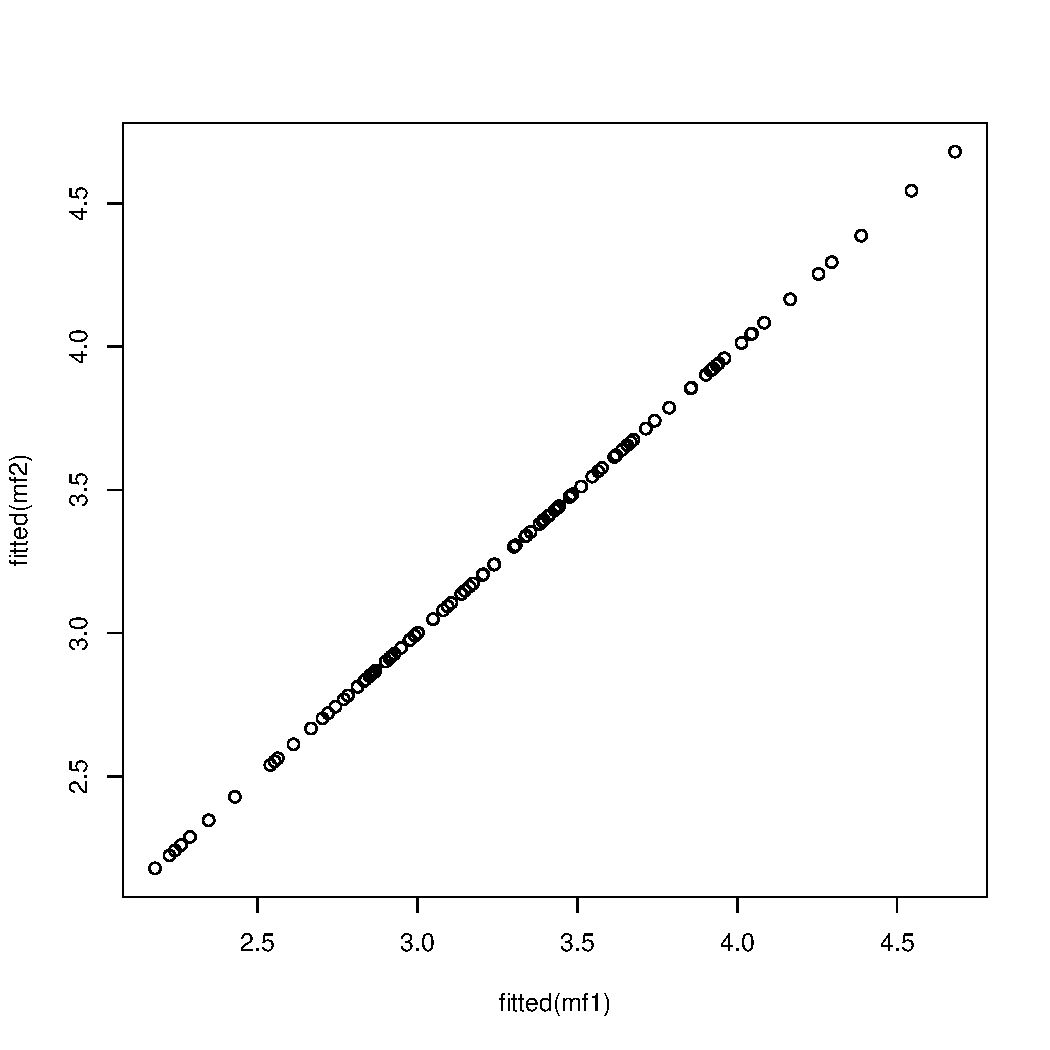
\includegraphics[width=\maxwidth]{figure/unnamed-chunk-13-1} 

\end{knitrout}


\end{Exercise}
\begin{Answer}

\end{Answer}

\subsection{Turning long complicated code into a function}

\begin{Exercise}[difficulty=2, title={Turning a piece of code into a function}]
Tthe following piece of code simulate p-values for a random effect in a mixed model:
\begin{knitrout}
\definecolor{shadecolor}{rgb}{0.969, 0.969, 0.969}\color{fgcolor}\begin{kframe}
\begin{alltt}
\hlstd{RandomVariance} \hlkwb{<-} \hlnum{0}
\hlstd{sampsize} \hlkwb{<-} \hlnum{500}
\hlstd{nbblocks} \hlkwb{<-} \hlnum{30}
\hlstd{pvals} \hlkwb{<-} \hlkwd{vector}\hlstd{(}\hlkwc{length} \hlstd{=} \hlnum{1000}\hlstd{)}
\hlstd{altpvals} \hlkwb{<-} \hlkwd{vector}\hlstd{(}\hlkwc{length} \hlstd{=} \hlnum{1000}\hlstd{)}
\hlkwa{for} \hlstd{(i} \hlkwa{in} \hlnum{1}\hlopt{:}\hlnum{1000}\hlstd{)}
\hlstd{\{}
\hlstd{x} \hlkwb{<-} \hlkwd{rnorm}\hlstd{(sampsize,}\hlkwc{mean} \hlstd{=} \hlnum{4}\hlstd{,} \hlkwc{sd}\hlstd{=}\hlnum{0.25}\hlstd{)}
\hlstd{block} \hlkwb{<-} \hlkwd{sample}\hlstd{(}\hlkwc{x} \hlstd{=} \hlnum{1}\hlopt{:}\hlstd{nbblocks,} \hlkwc{size} \hlstd{= sampsize,} \hlkwc{replace} \hlstd{=} \hlnum{TRUE}\hlstd{)}
\hlstd{blockvalues} \hlkwb{<-} \hlkwd{rnorm}\hlstd{(}\hlkwc{n} \hlstd{= nbblocks,} \hlkwc{mean} \hlstd{=} \hlnum{0}\hlstd{,} \hlkwc{sd} \hlstd{=} \hlkwd{sqrt}\hlstd{(RandomVariance))}
\hlstd{y} \hlkwb{<-} \hlnum{8} \hlopt{-} \hlstd{x} \hlopt{+} \hlstd{blockvalues[block]} \hlopt{+} \hlkwd{rnorm}\hlstd{(sampsize,}\hlnum{0}\hlstd{,}\hlnum{1}\hlstd{)}
\hlstd{dat} \hlkwb{<-} \hlkwd{data.frame}\hlstd{(}\hlkwc{response} \hlstd{= y,} \hlkwc{predictor} \hlstd{= x,} \hlkwc{block}\hlstd{=block)}
\hlstd{lm0} \hlkwb{<-} \hlkwd{lm}\hlstd{(response} \hlopt{~} \hlnum{1} \hlopt{+} \hlstd{predictor,} \hlkwc{data}\hlstd{=dat)}
\hlstd{lmm0} \hlkwb{<-} \hlkwd{lmer}\hlstd{(response} \hlopt{~} \hlnum{1} \hlopt{+} \hlstd{predictor} \hlopt{+} \hlstd{(}\hlnum{1}\hlopt{|}\hlstd{block),} \hlkwc{data}\hlstd{=dat )}
\hlstd{(LRT0} \hlkwb{<-} \hlkwd{anova}\hlstd{(lmm0, lm0))} \hlcom{#mixed model must come first!}
\hlstd{pvals[i]} \hlkwb{<-} \hlstd{LRT0}\hlopt{$}\hlstd{`Pr(>Chisq)`[}\hlnum{2}\hlstd{]} \hlcom{# the p-value}
\hlstd{altpvals[i]} \hlkwb{<-} \hlnum{1}\hlopt{-}\hlkwd{pchisq}\hlstd{(LRT0}\hlopt{$}\hlstd{Chisq[}\hlnum{2}\hlstd{],}\hlnum{0.5}\hlstd{)} \hlcom{# a better p-value}
\hlstd{\}}
\hlstd{pvals}
\hlstd{altpvals}
\end{alltt}
\end{kframe}
\end{knitrout}

Turn this into a function were the arguments will let you control:
  \begin{itemize}
    \item The value of the simulated variance (RandomVariance)
    \item The number of simulations (above it is fixed to 1000)
    \item (optionally) The sample size and number of random levels (blocks)
  \end{itemize}
And output:
  \begin{itemize}
    \item A vector of standard p-values from the LRT
    \item (optionally) a vector of "alternative" p-values (from the hand-made Chi-square)
    \item (optionally) histograms of the distribution of p-values
  \end{itemize}

\end{Exercise}
\begin{Answer}
\begin{knitrout}
\definecolor{shadecolor}{rgb}{0.969, 0.969, 0.969}\color{fgcolor}\begin{kframe}
\begin{alltt}
\hlstd{Fpvalsimul} \hlkwb{<-} \hlkwa{function}\hlstd{(}\hlkwc{RandomVariance} \hlstd{=} \hlnum{0}\hlstd{,}
                       \hlkwc{sampsize} \hlstd{=} \hlnum{500}\hlstd{,}
                       \hlkwc{nbblocks} \hlstd{=} \hlnum{30}\hlstd{,}
                       \hlkwc{nsimuls} \hlstd{=} \hlnum{100}\hlstd{)\{}
  \hlkwd{require}\hlstd{(lme4)}
\hlstd{pvals} \hlkwb{<-} \hlkwd{vector}\hlstd{(}\hlkwc{length} \hlstd{= nsimuls)}
\hlstd{altpvals} \hlkwb{<-} \hlkwd{vector}\hlstd{(}\hlkwc{length} \hlstd{= nsimuls)}
\hlkwa{for} \hlstd{(i} \hlkwa{in} \hlnum{1}\hlopt{:}\hlstd{nsimuls)}
\hlstd{\{}
\hlstd{x} \hlkwb{<-} \hlkwd{rnorm}\hlstd{(sampsize,}\hlkwc{mean} \hlstd{=} \hlnum{4}\hlstd{,} \hlkwc{sd}\hlstd{=}\hlnum{0.25}\hlstd{)}
\hlstd{block} \hlkwb{<-} \hlkwd{sample}\hlstd{(}\hlkwc{x} \hlstd{=} \hlnum{1}\hlopt{:}\hlstd{nbblocks,} \hlkwc{size} \hlstd{= sampsize,} \hlkwc{replace} \hlstd{=} \hlnum{TRUE}\hlstd{)}
\hlstd{blockvalues} \hlkwb{<-} \hlkwd{rnorm}\hlstd{(}\hlkwc{n} \hlstd{= nbblocks,} \hlkwc{mean} \hlstd{=} \hlnum{0}\hlstd{,} \hlkwc{sd} \hlstd{=} \hlkwd{sqrt}\hlstd{(RandomVariance))}
\hlstd{y} \hlkwb{<-} \hlnum{8} \hlopt{-} \hlstd{x} \hlopt{+} \hlstd{blockvalues[block]} \hlopt{+} \hlkwd{rnorm}\hlstd{(sampsize,}\hlnum{0}\hlstd{,}\hlnum{1}\hlstd{)}
\hlstd{dat} \hlkwb{<-} \hlkwd{data.frame}\hlstd{(}\hlkwc{response} \hlstd{= y,} \hlkwc{predictor} \hlstd{= x,} \hlkwc{block}\hlstd{=block)}
\hlstd{lm0} \hlkwb{<-} \hlkwd{lm}\hlstd{(response} \hlopt{~} \hlnum{1} \hlopt{+} \hlstd{predictor,} \hlkwc{data}\hlstd{=dat)}
\hlstd{lmm0} \hlkwb{<-} \hlkwd{lmer}\hlstd{(response} \hlopt{~} \hlnum{1} \hlopt{+} \hlstd{predictor} \hlopt{+} \hlstd{(}\hlnum{1}\hlopt{|}\hlstd{block),} \hlkwc{data}\hlstd{=dat )}
\hlstd{(LRT0} \hlkwb{<-} \hlkwd{anova}\hlstd{(lmm0, lm0))} \hlcom{#mixed model must come first!}
\hlstd{pvals[i]} \hlkwb{<-} \hlstd{LRT0}\hlopt{$}\hlstd{`Pr(>Chisq)`[}\hlnum{2}\hlstd{]} \hlcom{# the p-value}
\hlstd{altpvals[i]} \hlkwb{<-} \hlnum{1}\hlopt{-}\hlkwd{pchisq}\hlstd{(LRT0}\hlopt{$}\hlstd{Chisq[}\hlnum{2}\hlstd{],}\hlnum{0.5}\hlstd{)} \hlcom{# a better p-value}
\hlstd{\}}
\hlstd{output} \hlkwb{<-} \hlkwd{list}\hlstd{(}\hlkwc{pvals}\hlstd{=pvals,} \hlkwc{altpvals}\hlstd{=altpvals)}
\hlkwd{par}\hlstd{(}\hlkwc{mfrow}\hlstd{=}\hlkwd{c}\hlstd{(}\hlnum{1}\hlstd{,}\hlnum{2}\hlstd{))}
\hlkwd{hist}\hlstd{(pvals);} \hlkwd{hist}\hlstd{(altpvals)}
\hlkwd{return}\hlstd{(output)}
\hlstd{\}}
\end{alltt}
\end{kframe}
\end{knitrout}
\end{Answer}


\section{Funny things}

\subsection{The dot-dot-dot}

\begin{Exercise}[difficulty=1, title={Understand the \texttt{\dots}}]
Consider these two functions:
\begin{knitrout}
\definecolor{shadecolor}{rgb}{0.969, 0.969, 0.969}\color{fgcolor}\begin{kframe}
\begin{alltt}
\hlstd{halfmean1} \hlkwb{<-} \hlkwa{function}\hlstd{(}\hlkwc{x}\hlstd{)}
\hlstd{\{}
  \hlkwd{mean}\hlstd{(x)}\hlopt{/}\hlnum{2}
\hlstd{\}}
\hlstd{halfmean2} \hlkwb{<-} \hlkwa{function}\hlstd{(}\hlkwc{x}\hlstd{,}\hlkwc{...}\hlstd{)}
\hlstd{\{}
  \hlkwd{mean}\hlstd{(x,...)}\hlopt{/}\hlnum{2}
\hlstd{\}}
\end{alltt}
\end{kframe}
\end{knitrout}

They behave the same way in the first case, but differently in the second:
\begin{knitrout}
\definecolor{shadecolor}{rgb}{0.969, 0.969, 0.969}\color{fgcolor}\begin{kframe}
\begin{alltt}
\hlstd{somedata} \hlkwb{<-} \hlkwd{c}\hlstd{(}\hlnum{10}\hlstd{,} \hlnum{25}\hlstd{,} \hlnum{NA}\hlstd{)}

\hlkwd{halfmean1}\hlstd{(somedata)}
\end{alltt}
\begin{verbatim}
## [1] NA
\end{verbatim}
\begin{alltt}
\hlkwd{halfmean2}\hlstd{(somedata)}
\end{alltt}
\begin{verbatim}
## [1] NA
\end{verbatim}
\begin{alltt}
\hlkwd{halfmean1}\hlstd{(somedata,} \hlkwc{na.rm}\hlstd{=}\hlnum{TRUE}\hlstd{)}
\end{alltt}


{\ttfamily\noindent\bfseries\color{errorcolor}{\#\# Error in halfmean1(somedata, na.rm = TRUE): unused argument (na.rm = TRUE)}}\begin{alltt}
\hlkwd{halfmean2}\hlstd{(somedata,} \hlkwc{na.rm}\hlstd{=}\hlnum{TRUE}\hlstd{)}
\end{alltt}
\begin{verbatim}
## [1] 8.75
\end{verbatim}
\end{kframe}
\end{knitrout}
What does \dots do?
\end{Exercise}
\begin{Answer}
\dots let you pass extra arguments to the function inside your function (but the extra arguments are passed to ALL functions inside, so be careful!)
\end{Answer}

\subsection{The \texttt{<<-} operator}

\begin{Exercise}[difficulty=1, title={Understand the \texttt{<<-}}]
We create to almost identical functions, f0 and f1 and add their output to an object \texttt{x}. Compare the output and explain what happens. What does \texttt{<<-} mean?

\begin{knitrout}
\definecolor{shadecolor}{rgb}{0.969, 0.969, 0.969}\color{fgcolor}\begin{kframe}
\begin{alltt}
\hlstd{f0} \hlkwb{<-} \hlkwa{function}\hlstd{(}\hlkwc{x}\hlstd{=}\hlnum{2}\hlstd{)\{}
  \hlstd{x} \hlkwb{<-} \hlstd{x}
  \hlstd{y} \hlkwb{<-} \hlstd{x}\hlopt{+}\hlnum{2}
  \hlkwd{return}\hlstd{(y)}
\hlstd{\}}

\hlstd{f1} \hlkwb{<-} \hlkwa{function}\hlstd{(}\hlkwc{x}\hlstd{=}\hlnum{2}\hlstd{)\{}
  \hlstd{x} \hlkwb{<<-} \hlstd{x}
  \hlstd{y} \hlkwb{<-} \hlstd{x}\hlopt{+}\hlnum{2}
  \hlkwd{return}\hlstd{(y)}
\hlstd{\}}

\hlstd{x} \hlkwb{<-} \hlkwd{rnorm}\hlstd{(}\hlnum{1000}\hlstd{)}
\hlkwd{f0}\hlstd{()}\hlopt{+}\hlstd{x}

\hlstd{x} \hlkwb{<-} \hlkwd{rnorm}\hlstd{(}\hlnum{1000}\hlstd{)}
\hlkwd{f1}\hlstd{()}\hlopt{+}\hlstd{x}
\end{alltt}
\end{kframe}
\end{knitrout}

\end{Exercise}

\begin{Answer}
The \texttt{<<-} operator breaks the borders of the function environment to assign a value to an object outside that function.
\end{Answer}


\subsection{Recursive functions}

\begin{Exercise}[difficulty=2, title={What does this function do?}]
Consider the following function and try to understand what it does. (code by Dr. Koen van Benthem)
\begin{knitrout}
\definecolor{shadecolor}{rgb}{0.969, 0.969, 0.969}\color{fgcolor}\begin{kframe}
\begin{alltt}
\hlstd{tree}\hlkwb{<-}\hlkwa{function}\hlstd{(}\hlkwc{x}\hlstd{,}\hlkwc{y}\hlstd{,}\hlkwc{l}\hlstd{,}\hlkwc{dir}\hlstd{,}\hlkwc{n}\hlstd{,}\hlkwc{nmax}\hlstd{)\{}
\hlkwa{if}\hlstd{(n}\hlopt{==}\hlnum{0}\hlstd{)\{}
\hlkwd{return}\hlstd{()}
\hlstd{\}}
\hlstd{pos}\hlkwb{<-}\hlkwd{round}\hlstd{(}\hlkwd{runif}\hlstd{(}\hlnum{1}\hlstd{,}\hlnum{1}\hlstd{,}\hlnum{199}\hlstd{))}
\hlstd{colour}\hlkwb{=}\hlkwd{rainbow}\hlstd{(}\hlnum{200}\hlstd{,}\hlkwc{start}\hlstd{=}\hlnum{0.2}\hlstd{,}\hlkwc{end}\hlstd{=}\hlnum{0.6}\hlstd{,}\hlkwc{v}\hlstd{=}\hlnum{0.6}\hlstd{)[pos]}
\hlkwd{lines}\hlstd{(}\hlkwd{c}\hlstd{(x,x}\hlopt{+}\hlstd{l}\hlopt{*}\hlkwd{sin}\hlstd{(dir)),}\hlkwd{c}\hlstd{(y,y}\hlopt{+}\hlstd{l}\hlopt{*}\hlkwd{cos}\hlstd{(dir)),}
      \hlkwc{lwd}\hlstd{=}\hlnum{20}\hlopt{*}\hlstd{(n}\hlopt{/}\hlstd{nmax),}\hlkwc{col}\hlstd{=colour)}
\hlstd{branches}\hlkwb{<-}\hlkwd{round}\hlstd{(}\hlkwd{runif}\hlstd{(}\hlnum{1}\hlstd{,}\hlnum{2}\hlstd{,}\hlnum{4}\hlstd{))}
\hlkwa{for}\hlstd{(i} \hlkwa{in} \hlnum{1}\hlopt{:}\hlstd{branches)\{}
\hlstd{angle}\hlkwb{<-}\hlstd{dir}\hlopt{+}\hlstd{(}\hlopt{-}\hlstd{pi}\hlopt{/}\hlnum{6}\hlstd{)}\hlopt{+}\hlstd{(pi}\hlopt{/}\hlnum{3}\hlstd{)}\hlopt{*}\hlstd{(i}\hlopt{-}\hlnum{1}\hlstd{)}\hlopt{/}\hlstd{(branches}\hlopt{-}\hlnum{1}\hlstd{)}
\hlstd{l2}\hlkwb{<-}\hlkwd{runif}\hlstd{(}\hlnum{1}\hlstd{,}\hlnum{0.7}\hlstd{,}\hlnum{0.85}\hlstd{)}\hlopt{*}\hlstd{l}
\hlkwd{tree}\hlstd{(x}\hlopt{+}\hlstd{l}\hlopt{*}\hlkwd{sin}\hlstd{(dir),y}\hlopt{+}\hlstd{l}\hlopt{*}\hlkwd{cos}\hlstd{(dir),l2,angle,n}\hlopt{-}\hlnum{1}\hlstd{,nmax)}
\hlstd{\}}
\hlstd{\}}
\end{alltt}
\end{kframe}
\end{knitrout}

You can run the function and see if you had guessed right:
\begin{knitrout}
\definecolor{shadecolor}{rgb}{0.969, 0.969, 0.969}\color{fgcolor}\begin{kframe}
\begin{alltt}
\hlkwd{plot}\hlstd{(}\hlnum{0}\hlstd{,}\hlnum{0}\hlstd{,}\hlkwc{type}\hlstd{=}\hlstr{"n"}\hlstd{,}\hlkwc{xlim}\hlstd{=}\hlkwd{c}\hlstd{(}\hlopt{-}\hlnum{10}\hlstd{,}\hlnum{10}\hlstd{),}\hlkwc{ylim}\hlstd{=}\hlkwd{c}\hlstd{(}\hlnum{0}\hlstd{,}\hlnum{10}\hlstd{),}
\hlkwc{xaxt}\hlstd{=}\hlstr{"n"}\hlstd{,}\hlkwc{yaxt}\hlstd{=}\hlstr{"n"}\hlstd{,}\hlkwc{ylab}\hlstd{=}\hlstr{""}\hlstd{,}\hlkwc{xlab}\hlstd{=}\hlstr{""}\hlstd{)}

\hlkwd{tree}\hlstd{(}\hlnum{0}\hlstd{,}\hlnum{0}\hlstd{,}\hlnum{2}\hlstd{,}\hlnum{0}\hlstd{,}\hlnum{8}\hlstd{,}\hlnum{12}\hlstd{)}
\end{alltt}
\end{kframe}
\includegraphics[width=\maxwidth]{figure/unnamed-chunk-21-1} 

\end{knitrout}

What is special about this function? Why should you be careful not to give large values to the parameters n? 
\end{Exercise}
\begin{Answer}
This is a self-referencing function, it calls itself! Each call to the function produces several new calls to the function, and so the number of times the function is called grows exponentially with the value of n. I do not recommend values above 12. That is a general problem to consider with recursive functions. 
\begin{knitrout}
\definecolor{shadecolor}{rgb}{0.969, 0.969, 0.969}\color{fgcolor}\begin{kframe}
\begin{alltt}
\hlstd{tree}\hlkwb{<-}\hlkwa{function}\hlstd{(}\hlkwc{x}\hlstd{,}\hlkwc{y}\hlstd{,}\hlkwc{l}\hlstd{,}\hlkwc{dir}\hlstd{,}\hlkwc{n}\hlstd{,}\hlkwc{nmax}\hlstd{)\{} \hlcom{# We define a function 'tree()'}
\hlcom{# x,y: start of tree, l: length of first branch, dir: direction}
\hlcom{# n and nmax: should be the same number: number of levels in the}
\hlcom{# tree.}
\hlcom{# An important escape argument, leave this out and the function}
\hlcom{# will run forever:}
\hlkwa{if}\hlstd{(n}\hlopt{==}\hlnum{0}\hlstd{)\{}
\hlkwd{return}\hlstd{()}
\hlstd{\}}
\hlcom{# Picking a colour at random using the rainbow function}
\hlcom{# (without this the code would also work, there would just be}
\hlcom{# no colors)}
\hlstd{pos}\hlkwb{<-}\hlkwd{round}\hlstd{(}\hlkwd{runif}\hlstd{(}\hlnum{1}\hlstd{,}\hlnum{1}\hlstd{,}\hlnum{199}\hlstd{))}
\hlstd{colour}\hlkwb{=}\hlkwd{rainbow}\hlstd{(}\hlnum{200}\hlstd{,}\hlkwc{start}\hlstd{=}\hlnum{0.2}\hlstd{,}\hlkwc{end}\hlstd{=}\hlnum{0.6}\hlstd{,}\hlkwc{v}\hlstd{=}\hlnum{0.6}\hlstd{)[pos]}
\hlcom{# Draw a line starting a (x,y) with length 'l' and in direction}
\hlcom{# (in radials) dir. On top of that, we make the width of the}
\hlcom{# line depend on how far the branch is from the stem.}
\hlkwd{lines}\hlstd{(}\hlkwd{c}\hlstd{(x,x}\hlopt{+}\hlstd{l}\hlopt{*}\hlkwd{sin}\hlstd{(dir)),}\hlkwd{c}\hlstd{(y,y}\hlopt{+}\hlstd{l}\hlopt{*}\hlkwd{cos}\hlstd{(dir)),}
      \hlkwc{lwd}\hlstd{=}\hlnum{20}\hlopt{*}\hlstd{(n}\hlopt{/}\hlstd{nmax),}\hlkwc{col}\hlstd{=colour)}
\hlcom{# Generate a random number that defines how many branches the}
\hlcom{# tree has at this point in the structure}
\hlstd{branches}\hlkwb{<-}\hlkwd{round}\hlstd{(}\hlkwd{runif}\hlstd{(}\hlnum{1}\hlstd{,}\hlnum{2}\hlstd{,}\hlnum{4}\hlstd{))}
\hlcom{# Now we go over the separate branches}
\hlkwa{for}\hlstd{(i} \hlkwa{in} \hlnum{1}\hlopt{:}\hlstd{branches)\{}
\hlcom{# to make sure not all branches point in the same direction,}
\hlcom{# we calculate a direction for the branch}
\hlstd{angle}\hlkwb{<-}\hlstd{dir}\hlopt{+}\hlstd{(}\hlopt{-}\hlstd{pi}\hlopt{/}\hlnum{6}\hlstd{)}\hlopt{+}\hlstd{(pi}\hlopt{/}\hlnum{3}\hlstd{)}\hlopt{*}\hlstd{(i}\hlopt{-}\hlnum{1}\hlstd{)}\hlopt{/}\hlstd{(branches}\hlopt{-}\hlnum{1}\hlstd{)}
\hlcom{# Also, we would like the later branches to be smaller than}
\hlcom{# the first one:}
\hlstd{l2}\hlkwb{<-}\hlkwd{runif}\hlstd{(}\hlnum{1}\hlstd{,}\hlnum{0.7}\hlstd{,}\hlnum{0.85}\hlstd{)}\hlopt{*}\hlstd{l}
\hlcom{# And finally the magic of recursion, we draw the new branch}
\hlcom{# simply by using theexact same function: the function 'tree'.}
\hlkwd{tree}\hlstd{(x}\hlopt{+}\hlstd{l}\hlopt{*}\hlkwd{sin}\hlstd{(dir),y}\hlopt{+}\hlstd{l}\hlopt{*}\hlkwd{cos}\hlstd{(dir),l2,angle,n}\hlopt{-}\hlnum{1}\hlstd{,nmax)}
\hlstd{\}}
\hlstd{\}}
\hlcom{# Now, to actually draw the tree, we first make an empty plot}
\hlkwd{plot}\hlstd{(}\hlnum{0}\hlstd{,}\hlnum{0}\hlstd{,}\hlkwc{type}\hlstd{=}\hlstr{"n"}\hlstd{,}\hlkwc{xlim}\hlstd{=}\hlkwd{c}\hlstd{(}\hlopt{-}\hlnum{10}\hlstd{,}\hlnum{10}\hlstd{),}\hlkwc{ylim}\hlstd{=}\hlkwd{c}\hlstd{(}\hlnum{0}\hlstd{,}\hlnum{10}\hlstd{),}
\hlkwc{xaxt}\hlstd{=}\hlstr{"n"}\hlstd{,}\hlkwc{yaxt}\hlstd{=}\hlstr{"n"}\hlstd{,}\hlkwc{ylab}\hlstd{=}\hlstr{""}\hlstd{,}\hlkwc{xlab}\hlstd{=}\hlstr{""}\hlstd{)}
\hlcom{# And then call the function tree() with the parameters we like}
\hlkwd{tree}\hlstd{(}\hlnum{0}\hlstd{,}\hlnum{0}\hlstd{,}\hlnum{2}\hlstd{,}\hlnum{0}\hlstd{,}\hlnum{8}\hlstd{,}\hlnum{8}\hlstd{)}
\end{alltt}
\end{kframe}
\includegraphics[width=\maxwidth]{figure/unnamed-chunk-22-1} 

\end{knitrout}
\end{Answer}

\begin{Exercise}[difficulty=3, title={Find a mistake in a family tree (Challenging!)}]
For this exercise you will need to download a file as follows: 
\begin{knitrout}
\definecolor{shadecolor}{rgb}{0.969, 0.969, 0.969}\color{fgcolor}\begin{kframe}
\begin{alltt}
\hlkwd{download.file}\hlstd{(}\hlkwc{url}\hlstd{=}\hlstr{"https://raw.githubusercontent.com/
timotheenivalis/RSB-R-Stats-Biology/master/04.Functions/wrongpedigree.csv"}\hlstd{,}
\hlkwc{destfile} \hlstd{=} \hlstr{"wrongpedigree.csv"}\hlstd{)}

\hlstd{ped} \hlkwb{<-} \hlkwd{read.csv}\hlstd{(}\hlstr{"wrongpedigree.csv"}\hlstd{,} \hlkwc{stringsAsFactors} \hlstd{=} \hlnum{FALSE}\hlstd{)}
\end{alltt}
\end{kframe}
\end{knitrout}

The file \texttt{wrongpedigree.csv} contains a pedigree (a family tree) containing a mistake: a function we tried to apply on this data set informed us that the family tree was impossible without more information. We suspect that we have assigned an individual as its own ancestor (this can happen with genetic reconstruction of parentage). Use a self-referencing function to scan the tree and find where the problem is.
\end{Exercise}
\begin{Answer}
I found a solution using two functions: a recursive one, and one going using a for loop to go across incidivuals. Clearly that is not efficient. Feel free to think of a better way!

\begin{knitrout}
\definecolor{shadecolor}{rgb}{0.969, 0.969, 0.969}\color{fgcolor}\begin{kframe}
\begin{alltt}
\hlstd{checkp} \hlkwb{<-} \hlkwa{function}\hlstd{(}\hlkwc{iniind}\hlstd{,} \hlkwc{focalind}\hlstd{,} \hlkwc{ped}\hlstd{,} \hlkwc{level}\hlstd{=}\hlnum{1}\hlstd{,} \hlkwc{maxlevel}\hlstd{=}\hlnum{3}\hlstd{,}
                   \hlkwc{idname} \hlstd{=} \hlstr{"animal"}\hlstd{)}
\hlstd{\{}
  \hlstd{parents} \hlkwb{<-} \hlstd{ped[}\hlkwd{as.character}\hlstd{(ped[,idname])}\hlopt{==}
                   \hlkwd{as.character}\hlstd{(focalind),}\hlkwd{c}\hlstd{(}\hlnum{2}\hlstd{,}\hlnum{3}\hlstd{)]}
  \hlstd{circular} \hlkwb{<-} \hlnum{0}
  \hlkwa{for}\hlstd{(j} \hlkwa{in} \hlnum{1}\hlopt{:}\hlnum{2}\hlstd{)}
  \hlstd{\{}
    \hlkwa{if}\hlstd{(}\hlopt{!}\hlkwd{is.na}\hlstd{(parents[j]))}
    \hlstd{\{}
      \hlkwa{if}\hlstd{(}\hlkwd{as.character}\hlstd{(iniind)}\hlopt{==}\hlkwd{as.character}\hlstd{(parents[j]))}
      \hlstd{\{}
        \hlstd{circular} \hlkwb{<-} \hlstd{circular}\hlopt{+}\hlnum{1}
        \hlkwd{warning}\hlstd{(}\hlstr{"Individual"}\hlstd{, iniind,} \hlstr{" is its own ancestor at level "}\hlstd{,}
                \hlstd{level,}  \hlstr{" (pair "}\hlstd{, parents[}\hlnum{1}\hlstd{],}\hlstr{";"}\hlstd{, parents[}\hlnum{2}\hlstd{],} \hlstr{")"}\hlstd{)}
      \hlstd{\}}\hlkwa{else}\hlstd{\{}
        \hlkwa{if}\hlstd{(level}\hlopt{<}\hlstd{maxlevel)}
        \hlstd{\{level} \hlkwb{<-} \hlstd{level}\hlopt{+}\hlnum{1}
        \hlstd{circular} \hlkwb{<-} \hlstd{circular} \hlopt{+} \hlkwd{checkp}\hlstd{(}\hlkwc{iniind}\hlstd{=iniind,} \hlkwc{focalind}\hlstd{=parents[j],}
                                      \hlkwc{ped} \hlstd{= ped,} \hlkwc{level}\hlstd{=level)}
        \hlstd{\}}
      \hlstd{\}}
    \hlstd{\}}
  \hlstd{\}}
  \hlkwd{return}\hlstd{(circular)}
\hlstd{\}}
\end{alltt}
\end{kframe}
\end{knitrout}

\begin{knitrout}
\definecolor{shadecolor}{rgb}{0.969, 0.969, 0.969}\color{fgcolor}\begin{kframe}
\begin{alltt}
\hlstd{checkpedwrap} \hlkwb{<-} \hlkwa{function}\hlstd{(}\hlkwc{ped}\hlstd{,} \hlkwc{idname}\hlstd{=}\hlstr{"animal"}\hlstd{,} \hlkwc{maxlevel}\hlstd{=}\hlnum{3}\hlstd{)}
\hlstd{\{}
  \hlstd{ped}\hlopt{$}\hlstd{circularity} \hlkwb{<-} \hlnum{NA}
  \hlkwa{for} \hlstd{(i} \hlkwa{in} \hlnum{1}\hlopt{:}\hlkwd{nrow}\hlstd{(ped))}
  \hlstd{\{}
    \hlstd{ped}\hlopt{$}\hlstd{circularity[i]} \hlkwb{<-} \hlkwd{checkp}\hlstd{(}\hlkwc{iniind}\hlstd{=ped[i, idname],}
                                 \hlkwc{focalind} \hlstd{= ped[i, idname],}
                                 \hlkwc{ped}\hlstd{=ped,} \hlkwc{level} \hlstd{=}\hlnum{1}\hlstd{,}
                                 \hlkwc{maxlevel}\hlstd{=maxlevel,} \hlkwc{idname}\hlstd{=idname)}
  \hlstd{\}}
  \hlkwd{return}\hlstd{(ped)}
\hlstd{\}}
\end{alltt}
\end{kframe}
\end{knitrout}


\begin{knitrout}
\definecolor{shadecolor}{rgb}{0.969, 0.969, 0.969}\color{fgcolor}\begin{kframe}
\begin{alltt}
\hlstd{ped} \hlkwb{<-} \hlkwd{read.csv}\hlstd{(}\hlstr{"wrongpedigree.csv"}\hlstd{,} \hlkwc{stringsAsFactors} \hlstd{=} \hlnum{FALSE}\hlstd{)}
\end{alltt}


{\ttfamily\noindent\color{warningcolor}{\#\# Warning in file(file, "{}rt"{}): cannot open file 'wrongpedigree.csv': No such file or directory}}

{\ttfamily\noindent\bfseries\color{errorcolor}{\#\# Error in file(file, "{}rt"{}): cannot open the connection}}\begin{alltt}
\hlstd{pedchecked} \hlkwb{<-} \hlkwd{checkpedwrap}\hlstd{(}\hlkwc{ped}\hlstd{=ped,} \hlkwc{idname} \hlstd{=} \hlstr{"animal"}\hlstd{,} \hlkwc{maxlevel} \hlstd{=} \hlnum{3}\hlstd{)}
\end{alltt}


{\ttfamily\noindent\bfseries\color{errorcolor}{\#\# Error in checkpedwrap(ped = ped, idname = "{}animal"{}, maxlevel = 3): object 'ped' not found}}\end{kframe}
\end{knitrout}
\end{Answer}


\end{document}
